\documentclass[12pt,]{article}
\usepackage{lmodern}
\usepackage{amssymb,amsmath}
\usepackage{ifxetex,ifluatex}
\usepackage{fixltx2e} % provides \textsubscript
\ifnum 0\ifxetex 1\fi\ifluatex 1\fi=0 % if pdftex
  \usepackage[T1]{fontenc}
  \usepackage[utf8]{inputenc}
\else % if luatex or xelatex
  \ifxetex
    \usepackage{mathspec}
  \else
    \usepackage{fontspec}
  \fi
  \defaultfontfeatures{Ligatures=TeX,Scale=MatchLowercase}
\fi
% use upquote if available, for straight quotes in verbatim environments
\IfFileExists{upquote.sty}{\usepackage{upquote}}{}
% use microtype if available
\IfFileExists{microtype.sty}{%
\usepackage{microtype}
\UseMicrotypeSet[protrusion]{basicmath} % disable protrusion for tt fonts
}{}
\usepackage[margin=1in]{geometry}
\usepackage{hyperref}
\hypersetup{unicode=true,
            pdftitle={External Debt and Currency Crisis in Emerging Markets},
            pdfauthor={New Group Project},
            pdfborder={0 0 0},
            breaklinks=true}
\urlstyle{same}  % don't use monospace font for urls
\usepackage{graphicx,grffile}
\makeatletter
\def\maxwidth{\ifdim\Gin@nat@width>\linewidth\linewidth\else\Gin@nat@width\fi}
\def\maxheight{\ifdim\Gin@nat@height>\textheight\textheight\else\Gin@nat@height\fi}
\makeatother
% Scale images if necessary, so that they will not overflow the page
% margins by default, and it is still possible to overwrite the defaults
% using explicit options in \includegraphics[width, height, ...]{}
\setkeys{Gin}{width=\maxwidth,height=\maxheight,keepaspectratio}
\IfFileExists{parskip.sty}{%
\usepackage{parskip}
}{% else
\setlength{\parindent}{0pt}
\setlength{\parskip}{6pt plus 2pt minus 1pt}
}
\setlength{\emergencystretch}{3em}  % prevent overfull lines
\providecommand{\tightlist}{%
  \setlength{\itemsep}{0pt}\setlength{\parskip}{0pt}}
\setcounter{secnumdepth}{0}
% Redefines (sub)paragraphs to behave more like sections
\ifx\paragraph\undefined\else
\let\oldparagraph\paragraph
\renewcommand{\paragraph}[1]{\oldparagraph{#1}\mbox{}}
\fi
\ifx\subparagraph\undefined\else
\let\oldsubparagraph\subparagraph
\renewcommand{\subparagraph}[1]{\oldsubparagraph{#1}\mbox{}}
\fi

%%% Use protect on footnotes to avoid problems with footnotes in titles
\let\rmarkdownfootnote\footnote%
\def\footnote{\protect\rmarkdownfootnote}

%%% Change title format to be more compact
\usepackage{titling}

% Create subtitle command for use in maketitle
\newcommand{\subtitle}[1]{
  \posttitle{
    \begin{center}\large#1\end{center}
    }
}

\setlength{\droptitle}{-2em}

  \title{External Debt and Currency Crisis in Emerging Markets}
    \pretitle{\vspace{\droptitle}\centering\huge}
  \posttitle{\par}
    \author{New Group Project}
    \preauthor{\centering\large\emph}
  \postauthor{\par}
      \predate{\centering\large\emph}
  \postdate{\par}
    \date{April 29, 2019}

\usepackage{setspace}\doublespacing

\begin{document}
\maketitle

\textbf{Members:}

\begin{itemize}
  \itemsep-.6em
  \item Liumin Chen (NetID: lc1077) - email: lc1077@georgetown.edu\
  \item Tingjie  Meng (NetID: tm1305) - email: tm1305@georgetown.edu\
\end{itemize}

\textbf{Github Repository:}
\url{https://github.com/TingjieMeng/New-Group-Project}

\section{Problem Statement}\label{problem-statement}

Debts and credits are crucial both for the expansion of businesses and
for economic development. However, when the growth of debts outpaces the
growth of income, debts become a time bomb triggering crises. There are
two types of debts: domestic debts denominated in the domestic currency
and external debts denominated in foreign currencies. The history of
financial crises tells us that countries with a high level of external
debt are especially vulnerable to capital outflows and thus exchange
rate fluctuations. As Ray Dalio describes in , such an event is called
an inflationary depression.

Classic examples of a deflationary depression are the Tukish currency
crises in the early 2000s and 2018. Since the 1980s, Turkey has been
heavily dependent on foreign investments to fund its huge current
account deficits, especially in the capital-intensive construction
sector. Thus its economy is fragile to any internal or external shock
that can lead to foreign capital outflow on a large scale. In 2001,
foreign investors quickly withdrew capital from Turkey amid political
tensions and tightening fiscal policies by the Turkish government, which
caused the value of Turkish lira to plunge. The history repeats itself.
In 2018, due to domestic instability and tightening monetary policies
from major central banks, Turkey saw a year-over-year decline of foreign
investments by 9,500 basis points. Without sufficient foreign capital to
support its weak economy, the Turkish lira soon began drastically losing
value, leaving many companies unable to serve their foreign currency
debts.

Our project focuses on studying the link between external debt and
currency crisis in Emerging Market Economies (EME). As shown in Turkey's
crises, over-dependence on external financing can be extremely dangerous
for EMEs in the long run. However, EMEs typically face difficulties in
issuing debts in local currency because their local financial markets
are underdeveloped. Thus they are more likely to hold a significant
portion of external debt in the total debt portfolio compared to
developed economies. Specifically, we explore factors that strengthen or
weaken the link between external debt and currency crisis in EMEs and
use the patterns we find to predict the possibility of a currency crisis
happening in future years. Our findings can serve as policy guidance for
external debt management for central bank policymakers in emerging
markets.

\section{Research Design}\label{research-design}

\subsection{testable hypothesis}\label{testable-hypothesis}

Our main hypothesis that countries who have borrowed excessively in
foreign currency are more prone to currency crisis risks. Sufficient
foreign reserves, a stable political regime, and a strong economy make
countries more resilient against currency depreciation risks. Currency
crises are more likely to happen when the U.S. Federal Reserve increases
the interst rate because that creates more incentives for investors to
bring money from EMEs back into the United States.

\subsection{dataset}\label{dataset}

A set of time series data covering 46 developing countries from 1990 to
2015

\subsection{data source}\label{data-source}

Data sources for this study are as follows: the World Bank Open Data,
the International Monetary Fund (IMF) Open Data, and the Polity IV
Project conducted by the Center for Systemic Peace. All three data
sources are publicly available. The World Bank and IMF APIs can be
installed in R, and the Polity IV Project data can be conveniently
downloaded as a csv package.

\subsection{variable description}\label{variable-description}

Dependent variable: possibility of a currency crisis happening, defined
as a nominal depreciation of 15\% within a year Independent variable of
interest: externaldebt/GNI Control variable: GDP per capita, level of
democracy, US 3-month treasury yield, foreign reserves/total external
debt

\section{Methods}\label{methods}

\subsection{data visualization}\label{data-visualization}

Data visualization is used for getting a general understanding of the
relationships between independent variables and dependent variables. It
is also used as case studies of individual countries that experience a
classic pattern of currency crises.

\subsection{mixed-effect logit model}\label{mixed-effect-logit-model}

The logit model in parameterization form is as follows. It is used for
modelling the probability of a currency crisis happening given all
variables. Pr(Currency Crisis = 1) = φ(β0 + β1(External debt to GNI)i,t
+ β2(Polity2)i,t + β3(US 3m yield)i + β4(lag GDP per capita)i,t + β5(lag
reserves to external debt)i,t + yeari + countryt + εi,t) -------- ??to
be shared with professor

\subsection{machine learning
techniques}\label{machine-learning-techniques}

Machine learning here is used for predicting the classification. We use
several models including K nearest neighbours, CART, and Random Forest.
After comparison, we choose the one model specification with the most
accuracy.

\subsection{GENERATE DEPENDENT VARIABLE
(DUMMY)}\label{generate-dependent-variable-dummy}

\subsection{GENERATE INDEPENDENT LAG
VARIABLES}\label{generate-independent-lag-variables}

summary of statistics: describe the variables

\section{Results}\label{results}

\subsection{data visualization}\label{data-visualization-1}

creat df1 to select only China, Argentina, Brazil, Romania, Russia
Federation, Sierra Leone, Thailand, Turkey and South Africa. df1 is used
to create graph1. display the external debt/gni by 11 countries

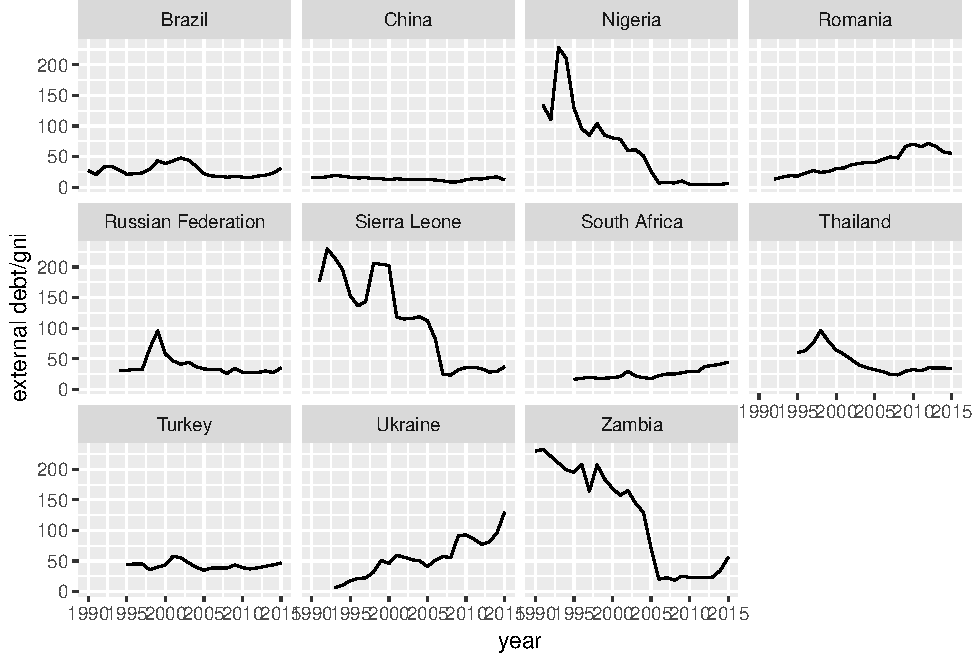
\includegraphics{Final_Work_Knit_files/figure-latex/unnamed-chunk-36-1.pdf}

Is it the higher the external debt, the more often currency crisis
happened? -yes, for Nigeria,Zambia,Thailand,Sierra Leoone.

multicollinearity: see the relationship between control variable: polity
score and gdp per capita display polity scores by countries:

display GDP per capita by countries

multicolinear? No. multicolinearity doesn't seem to exist. it make
sense: Nigeria, Romania -\textgreater{} The more ``democratic'', the
higher lagged gdp per capita not make sense: China, Brazil,Russia,
Ukraine, Sierra Leone, South Africa, Thailand, Turkey 1) The polity
score might not a strong factor reflecting political stability 2) The
polity score might not be strongly asscoiated with some countries'
currency crisis.

external shock: How U.S. interest rate influence EMEs' currency crisis?

Count the number of currency crisis of all selected countries by years

Display the U.S. interest rate by years

The trends of US interest rate and \# of countries undergoing currency
crisis appear to move in the same direction approximately. US interest
rate as an external shock has an impact on EMEs' currency crisis.

polity score and currency crisis by country: no direct relationship
found

The lower the foreign reserves, the more currency crisis happened.
strong relationship!

\subsection{LOGIT REGRESSION}\label{logit-regression}

\subsection{mixed-effect logit model}\label{mixed-effect-logit-model-1}

The logit model shows that there is a positive correlation between our
independent variable of interest and the dependent variable, and such
correlation is statistically significant at the 0.1\% level. This
supports our main hypothesis that countries who have borrowed
excessively in foreign currency are more prone to currency crisis risks.
In terms of control variables, the model shows a negative correlation
between the ratio of foreign reserves to a country's total external debt
in the previous year and the dependent variable. There is also a
negative correlation between GDP per capita in the previous year and the
probability of a currency crisis happening. However, the correlations
for both these two control variables are not statistically significant.
There is a positive correlation between US 3-month treasury yield and
the dependent variable, but again this correlation is not significant.
Generally, our finding is consistent with our theory, that countries
with stronger economies (higher GDP per capita) and sufficient foreign
reserves are more resilient against currency crises. Besides, in terms
of external factors, currency risks are particularly high during times
when the US Federal Reserve sets the interest rate high.\\
In our hypothesis, countries which have higher polity scores typically
have more transparent and efficient public management systems. That
enables those countries to deal with exchange rate problems more
effectively. However, the positive coefficient for polity score shown
here is in contrast with our expectation. This is most likely due to the
dataset issue, that the polity score is not the best indicator for level
of democracy. Countries like China and Brazil have low polity scores but
have stable exchange rates. There is no good equivalent to R-squared for
logistic regression models. One alternative is to look at the log
likelihood, which is -306.2 in this case. Another alternative is to look
at the AIC, which is 628.4 here. Both the log likelihood and AIC are
relative measures of model fit. A lower value of the AIC or higher value
of log likelihood suggests a relatively ``better'' model.

\subsection{MACHINE LEARNING}\label{machine-learning}

We split the data into a training and test dataset, partitioning data
before 2014 into the training data, and holding out data in and after
2014 as a test set. normalize the scale. KNN, CART, RF, Compare the
output of all three models. \#\# Test the out-of-sample predictive
performance for the best performing model, which is mod2\_rf. use a
table to visualize the predictive capability. For the Random Forest
model, three most important variables are external debt to gni, lagged
gdp per capita, and lagged total reserves.

\section{Conclusion}\label{conclusion}

\subsection{Lessons Learned}\label{lessons-learned}

The first and most straightforward policy implication is that countries
should be cautious about their level of external debt, especially
emerging market economies (EME). Secondly, EMEs can take multiple
measures to increase thier resilience against currency crises.Those
include stocking foreign reserves, maintaining the credibility of
central banks in the international capital market, and developing a
strong economy. The third policy implication is that currency crisis
risks are particularly high in times of Fed rate hikes. This reminds
policymakers from national central banks and international organizations
like the IMF that EMEs' external debts need to be more closely monitored
in times of interest rate volatility.

\subsection{Next steps}\label{next-steps}

First, as mentioned in the results analysis part, polity score published
by Center for Systemic Peace measures the level of democracy, not the
political regime stability. That introduces bias into our model.
Besides, potentially there can be more variables to be included in the
model, like the economic structure and exchange rate regime. Third, our
dataset only includes data until 2015, which means that currency crises
in Turkey and Argentina in 2018 are not in our sample. In future
research, it will be meaningful to see if our findings remain the same
when a larger sample is used.


\end{document}
